\documentclass[10pt]{article}
\usepackage{geometry}
\usepackage{cancel}
\usepackage{graphicx}
\usepackage{sectsty}
\pagenumbering{gobble}
%sectionfont{\centering}
%\geometry{
%	letterpaper,
%	left= 0.1in,
%	right=0.1in,
%	top=0.1in,
%	bottom=0.1in
%}
\geometry{papersize={10in,12in}, left= 0.1in,
	right=0.1in,
	top=0.1in,
	bottom=0.1in}
\usepackage{amssymb,amsmath}
\begin{document}
\section*{Model}
\[\hat{y}=11.9524+0.0029\cdot \hat{x},\quad \text{where}\quad  \hat{y}=\ln (\text{price})\text{ and } \hat{x} = \text{sqft\_living}^{0.78}  \]
\section*{Check Statistical Hypotheses of the Regression}
\subsection*{Linearity:}
\textbf{The Null Hypothesis:  The model is linearly predicted by the feature,\\
The Alternative Hypothesis:  The model is not linearly predicted by the feature.}\\
Our p-value for this model is \(p=0.877 > 0.05 = \alpha\). Thus, we don't have enough evidence to reject \textbf{The Null Hypothesis} and  we conclude that our model satisfies Linearity Assumption.
\subsection*{Normality Assumption for Errors}
To check Normality, I used the following checks:\\
\begin{minipage}{0.5\textwidth}
\begin{center}
	\textbf{QQ-Plot}\\
	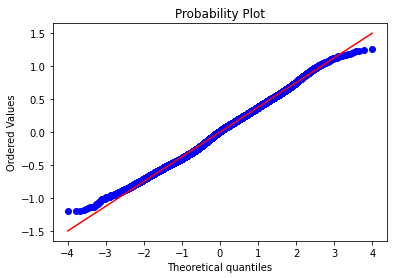
\includegraphics[width=2in,height=2in]{qq_plot_linear_model}
\end{center}%
\end{minipage}%
\begin{minipage}{0.5\textwidth}
	\begin{center}
		\textbf{DISTRIBUTIONS PLOT OF RESIDUALS}\\
		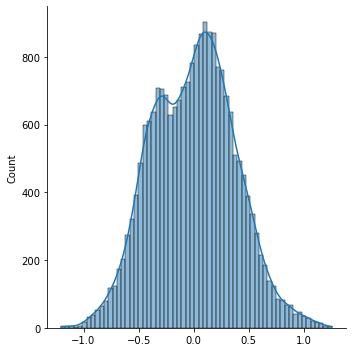
\includegraphics[width=2in,height=2in]{dist_plot_resid_linear_model}
	\end{center}%
\end{minipage}%
\\
I will, also, use D'Agostino Test for Normality:\\
\textbf{The Null Hypothesis:  The Residuals are normally distributed,\\
	The Alternative Hypothesis:  The Residuals are not normally distributed.}\\
Our p-value for this model is \(p=0.000 < 0.05 = \alpha\). Thus, we have enough evidence to reject the Null Hypothesis and conclude that D'Agostino Test tells us, that residuals are not normally distributed.\\
\vskip 0.1in
\noindent
\textbf{Conclusion:} Based on QQ-Plot, Distributions Plot, and D'Agostino Test, I conclude that the Distribution of Errors is not far away from Normal. Also, since we have a lot of observations Normality Assumption doesn't play a critical role, since Central Limit Theorem will apply in this case.
\subsection*{Constant Error Variance}
To if heteroscedasticity is present in the model, I will use Residual-vs-Predicted values plot and Breusch-Pagan test.
I look at at the Residual-vs-Predicted values plot first.
\begin{center}
	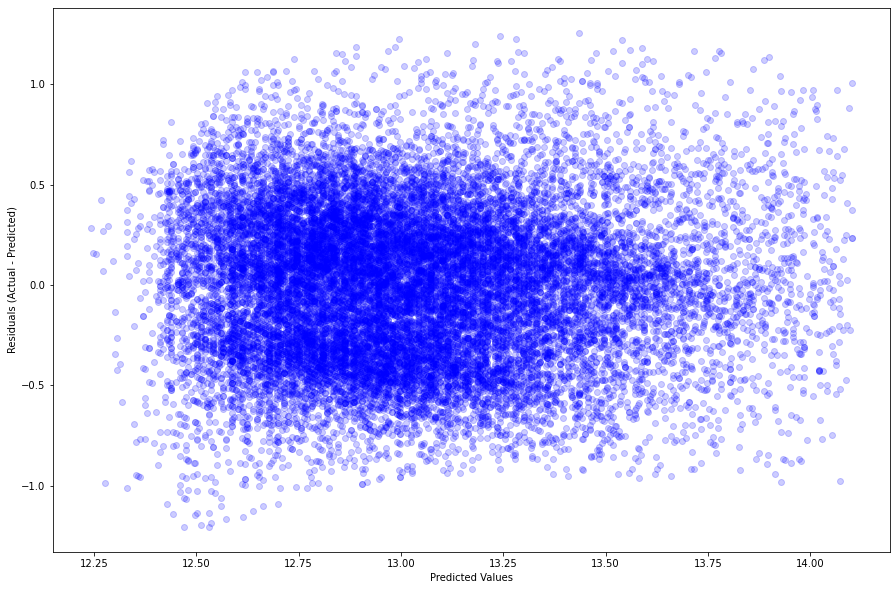
\includegraphics[width=3in]{residual_plot_linear_model}
\end{center}
Now, I will use Breusch-Pagan Test:\\
\textbf{The Null Hypothesis:  Homoscedasticity is present,\\
	The Alternative Hypothesis:  Homoscedasticity is not present (i.e. heteroscedasticity exists).}\\
Our p-value for this model is \(p=0.12609 \ge 0.05 = \alpha\). Thus, we don't have enough evidence to reject the Null Hypothesis and we conclude from Breusch-Pagan Test  , that we have don't have heteroscedasticity.\\
\textbf{Conclusion:} From the Residual-vs-Predicted values plot and  Breusch-Pagan Test, I conclude that we don't have Heteroscedasticity in our model.
\subsection*{Overall Conclusion:} I conclude that our model satisfies statistical assumptions for the regression model.
\end{document}
